\chapter{Overview of Rb magnetometer and apparatus}

\begin{itemize}
\item Purpose: Describe your experiment, focusing on the overall
  function, and providing some description of the individual
  components and their function.
\item Outline:
  \begin{itemize}
  \item Overview of experimental apparatus.  I think this is done by
    describing Figs.~\ref{fig:zerofield} and \ref{fig:pumpprobe}.
  \item Group Fig.~\ref{fig:pumpprobe} into major components and
    describe each one.  For example:
    \begin{itemize}
      \item ECDL and DAVLL
      \item Pump beam and AOM
      \item Probe beam and balanced polarimeter
      \item Cell
      \item Magnetic field system
        \begin{itemize}
        \item Shield arrangement
        \item Degaussing system
        \item Internal coil\underline{s}
        \end{itemize}
      \item DAQ
    \end{itemize}
  \item General operation is discussed in the next chapter.
  \end{itemize}
\end{itemize}

The purpose of this Chapter is to describe the experimental apparatus
used at UW.  I start with an explanation of the overall experiment.  I
then discuss each of the major components of the apparatus in more
detail.


% basic setup and its components,
%the dichroic atomic vapor laser lock (DAVLL), which is used for laser
%wavelength locking to the Cs absorption line will be
%discussed. Followed by an elucidation of the data acquisition (DAQ),

In Chapter~\ref{ch:characterization}, I will cover the initial
characterization of a few different modes of operation of the
magnetometer.  (As discussed in Chapter~\ref{ch:magnetometry}, there
are several different ways in which the magnetometer can be operated
dependent with different advantages and disadvantages to each.)

In Chapter~\ref{ch:results}, I discussed the advances made in the
understanding of the magnetometer performance, mostly in relation to
the development of the Free-Induction-Decay mode of operation.

%this section will be completed with the comparison of different
%possible operation modes of an atomic magnetometer and an introduction
%into the concepts of magnetometer uncertainties and the noise level of
%a measurement

\section{Overview}

\begin{figure}%[h]
\centering
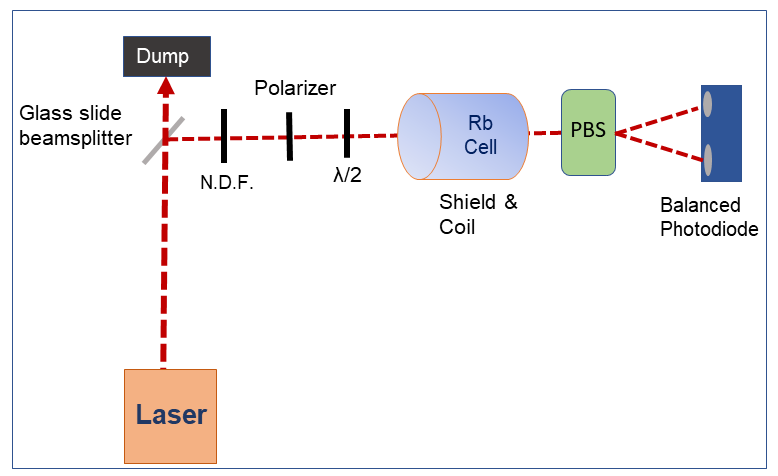
\includegraphics[width=0.8\textwidth]{figures/experimental_setup_zero_field}
\caption{Schematic diagram of experimental setup for zero field NMOR measurement (discussed in the text).\label{fig:zerofield}.}
\end{figure}
Fig.\ref{fig:zerofield} schematically depicts a top view of the Rb magnetometer, as it may be used for measurements of the magnetic field within a few hundred pT of zero.  This mode was used, for example, in Ref.~\cite{bib:nmor} to measure the axial magnetic shielding factor of
the passive magnetic shielding system.  In this thesis, this operation
mode was not normally used because we desired to develop the system
for larger magnetic fields.  But it is nonetheless instructive to
demonstrate the starting point of my thesis research.

  An external cavity diode laser produces light near the Rb D1 transition.  The laser is tuned near the $^{85}$Rb F=?? absorption minimum.  A microscope slide is used as a beamsplitter in order to divert a reduced power into the experiment.  The power is further reduced using neutral density filters (indicated by N.D.F. in Fig.~\ref{fig:zerofield}).  A linear polarizing sheet is oriented at a 45$^\circ$ angle relative to the vertical direction.  Since the laser
beam is polarized, this further reduces the power by a factor of two. The laser power after this point is normally in the range of 2-20~$\mu$W.  Small adjustments to the incident plane of polarization may be made by a $\lambda/2$ plate.  The beam then passes through a paraffin-coated cell containing Rb vapour.  The cell is within a
magnetic shielding and field generation system that produces a uniform field along the beam axis.  The plane of polarization of the laser
light will rotate slightly as it passes through the cell because of
non-linear magneto-optical effects.  A balanced polarimeter is used to
analyze the optical rotation of the laser light resulting from the
interaction of the laser light with the atoms in the cell.  The
polarimeter consists of a polarizing beam splitter (a Wollaston prism)
which splits the beam into its vertical and horizontal polarization
components.  Each component is sensed by a balanced photodiode which
outputs the difference in light intensities.  If the polarizer is set
at a 45$^\circ$ angle and aligned with the axis of the
$\lambda/2$-plate, and in the absence of any optical rotation, the
balanced photodiode would output zero volts.  If the plane of
polarization is rotated by passage through the cell, it will be sensed
 by the differential photodiode signal.  This is discussed further in Section~\ref{sec:Signal Processing}.
 
 Fig.~\ref{fig:pumpprobe}  shows the schematic layout of the apparatus used for studying the
non-linear magneto-optical effects with the amplitude modulated
light. This experimental setup is used in Forced oscillation scan and FID NMOR discussed in section \ref{sec:Forced-Oscillation Mode} and \ref{sec:FID}. In this work, a paraffin-coated vapor cell (about 5 cm long)
containing natural rubidium with stable isotopes $^{87}$Rb~ and~
$^{85}$Rb, is used as the magneto-optical sample. A semiconductor diode laser is the light source. The laser
wavelength ($\lambda=795$ nm) is precisely controlled by an external locking system.  The light beam is splited into pump and
probe beam using a microscope slide. The typical light power of the pump
beam is 40 $\mu$W and the typical light power of the probe beam is 20
$\mu$W.  Acousto Optic Modulator (AOM) is used to modulate the amplitude of the pump beam. The details of the working principle of AOM is discussed in section \ref{sec:AOM}. Upon passing through the AOM the pump beam is then passes through a lens to collimate. Before interact with the Rb cell pump beam then passes trough a N.D.F and polarizer to reduce the beam power. After that the linearly polarized light beam interact with Rb
atoms. 

The probe beam then passes through our vapour cell which sits inside the shield. Then the nonlinear Faraday rotation signals are analyzed by a balanced polarimeter.  A Wollaston prism is used to
split the beam into its perpendicular polarization axes which are then
analyzed individually by our photodiode. Our photodiode contains two
individual diodes and an internal differential amplifier which outputs the difference in diodes P1 - P2. A lock-in amplifier was used to detect the polarimetric signal and stored on a computer. Table \ref{table:laser power} shows the adjusted beam power at several positions of experimental setup.
\begin{figure}%[h]
\centering
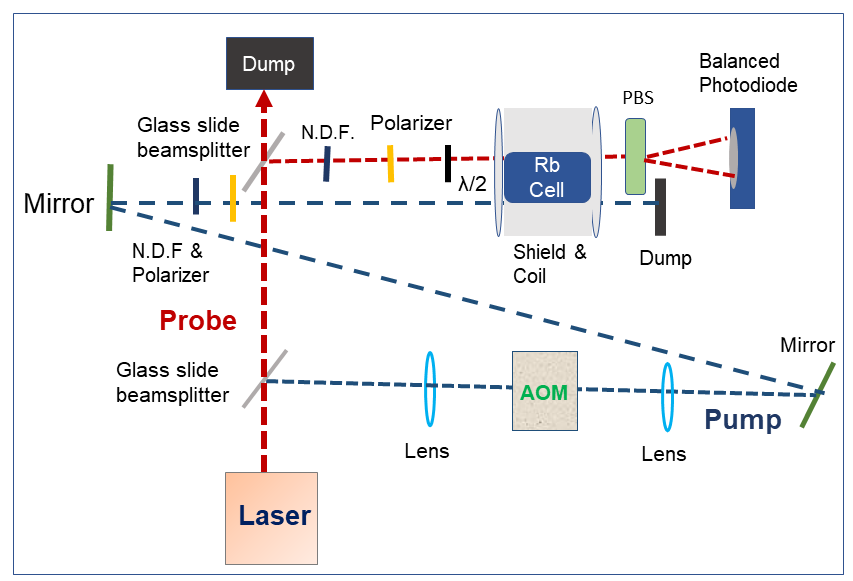
\includegraphics[width=0.95\linewidth]{figures/experimental_setup}
\caption{Schematic diagram of the experimental setup for measuring
  rotation of the polarization plane with amplitude modulated (AM)
  light. AOM stands for acousto optic modulator, $\lambda/2$ - half
  wave plate, N.D.F- neutral density filter, PBS- polarizing beam
  splitter.\label{fig:pumpprobe}}
\end{figure}
\section{External Cavity Diode Laser(ECDL)}
\bigskip
In our NMOR based optical magnetometry setup, laser light was provided by an external cavity diode laser. These kind of diodes are semiconductor diodes and thus vibration and shock resistant. They are also wavelength tunable. Besides that, external cavity diodes emit single mode laser light with a very narrow-band linewidth. A critical aspect of an ECDL is temperature control of the cavity, since the laser frequency depends on the cavity length and hence on the thermal expansion coefficient of the cavity material. Micrometer screws enable manual coarse tuning, while precise scans without mode hops are performed by a piezo actuator. This kind of grating stabilized diode lasers is especially advantageous for spectroscopy with the alkalines. Our Toptica DL-100 outputs a tunable wavelength near 795 nm with an output power $<100$ mW. The laser spot size is elliptical, and approximately 3 mm x 5 mm = $15 mm^2$.  The laser was typically tuned to the D1 (F = 3,2 2) absorption minimum and then adjusted to maximize optical rotation. 

\section{Dichroic Atomic Vapor Laser Lock (DAVLL)}

In order to control the laser frequency to a fraction of the Doppler-broadened linewidth of the relevant hyperfine atomic transition of the Rb D1-line, a frequency error signal is generated by taking usage of the Zeeman effect combined with circular dichroism of an atomic vapor which is exposed to a magnetic field \cite{doi:10.1063/1.3568824}. The generated error signal passes through zero crossings as the laser frequency coincident with the lock frequency. The schematic diagram of the apparatus used in  the DAVLL system has shown in Fig \ref{fig:DAVLL}. A linearly polarized probe beam is incident on a glass cell filled with Rb vapor surrounded by a set of permanent magnets. The wave vector of the light is parallel to the axis of the generated magnetic field by permanent magnets. After the interaction of the laser beam with the Rb cell, the beam passes through a quarter-wave plate before impinging on a polarizing beam splitter (PBS) or a Wollaston prism. The linearly polarized beam incident can be split into two orthogonal circularly polarized beams. A set of photodiodes are used to detect the intensity of the right and left circularly polarized beams. Both of the photodiodes are attached to a polarimeter board which is used to measure the difference in signals and amplifies it. A Tektronix TDS2024 oscilloscope is used for monitoring each photodiode signal as well as the difference output. The signal is then fed into a PID controller which finally controls the laser diode current corresponding to a certain laser frequency.
\begin{figure}[h]
\centering
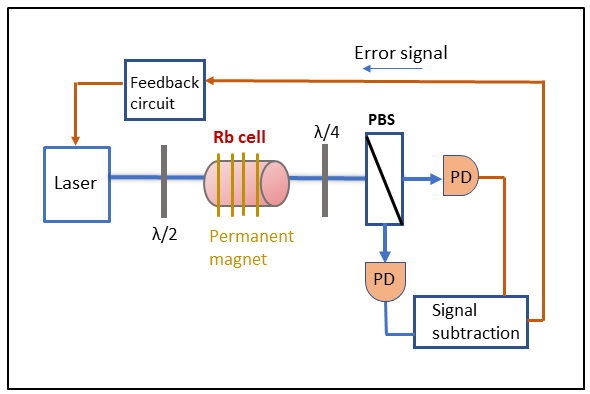
\includegraphics[width=0.8\linewidth]{figures/DAVLL}
\caption{Schematic diagram of experimental setup for characterizing the DAVLL . PBS- polarizing beam splitter, PD- photodiode.\label{fig:DAVLL}}
\end{figure}
\section{Laser tuning and locking}
In order to polarize atoms by optical pumping, it's important to tune the laser properly to expected transition line.
Setting the laser temperature correctly is one of the important parts to achieve good tuning . First we need to turn on the temperature control panel and then it’s easy to adjust laser temperature manually by tuning the knob of temperature control panel. For our tune the laser temperature is set to 20.1 $\degree$c. For good tuning it is also important to set the laser current which corresponds to the emission of laser light with a wavelength matching the absorption line of the Rb atom. This is usually done by a DAVLL scan so it's necessary to make sure the DAVLL optical setup is done correctly. An oscilloscope is used to observe the output of the differential amplifier. Trigger the scope on the trigger output on the scan control (SC) panel.
Laser current can be controlled by adjusting the current control knob until the spectral structure of $^{85}Rb$ appears (see Fig \ref{fig:laser tune}). we need to keep adjusting the current control knob until a maximum symmetry between the upsweep and downsweep portions is achieved. After that by adjusting the knob of scan control panel we can zoom in the structure and set the trigger to steep of the absorption minima. 
\begin{figure}[h]
\centering
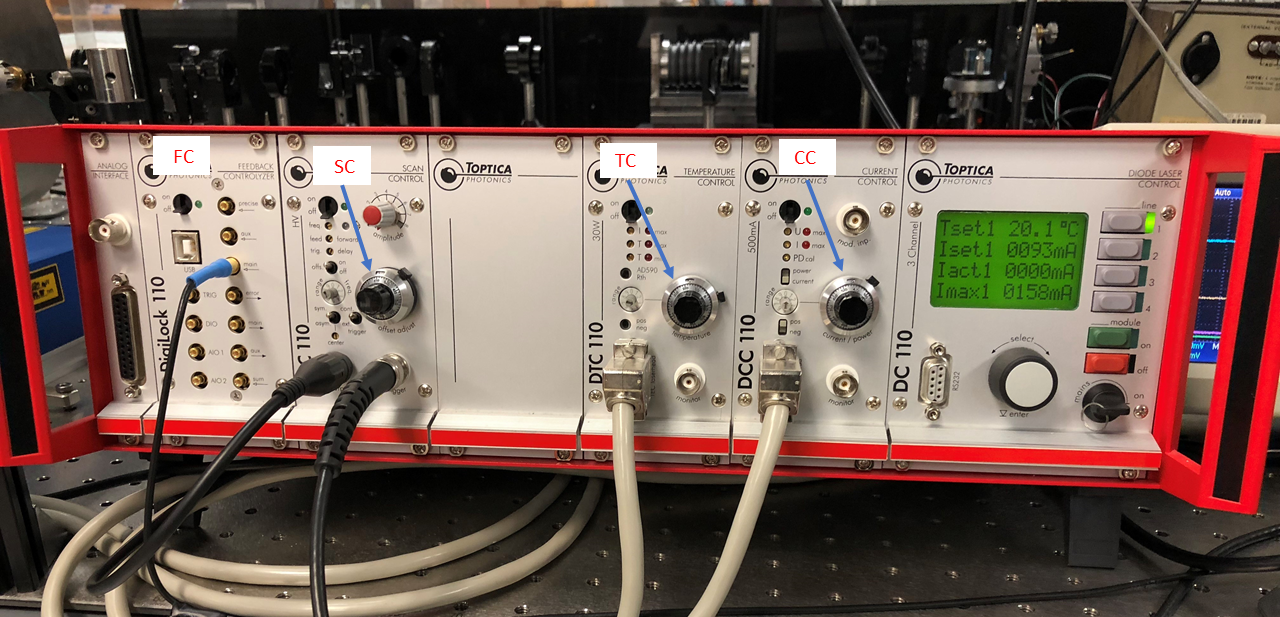
\includegraphics[width=0.8\linewidth]{figures/laser_control_}
\caption{Diode laser controller unit consist of analog current control module (CC), scan control module (SC),low-noise temperature control module (TC), feedback controlyzer (FC) and Diode Laser Controller display .\label{fig:laser controller}}
\end{figure}

Digilock 110 feedback controlyzer(FC) is used for laser locking. The DigiLock 110 is an up-to-date digital hardware allows to implement the scan generator, PID controllers and optional frequency modulation techniques all into one plug in module. It offers graphical user interface(see Fig \ref{fig:digilock}) running on a PC makes the procedure of laser locking enormously easy. Different important features are also available in this module for analyzing and optimizing the control system.
 \begin{figure}[h]
\centering
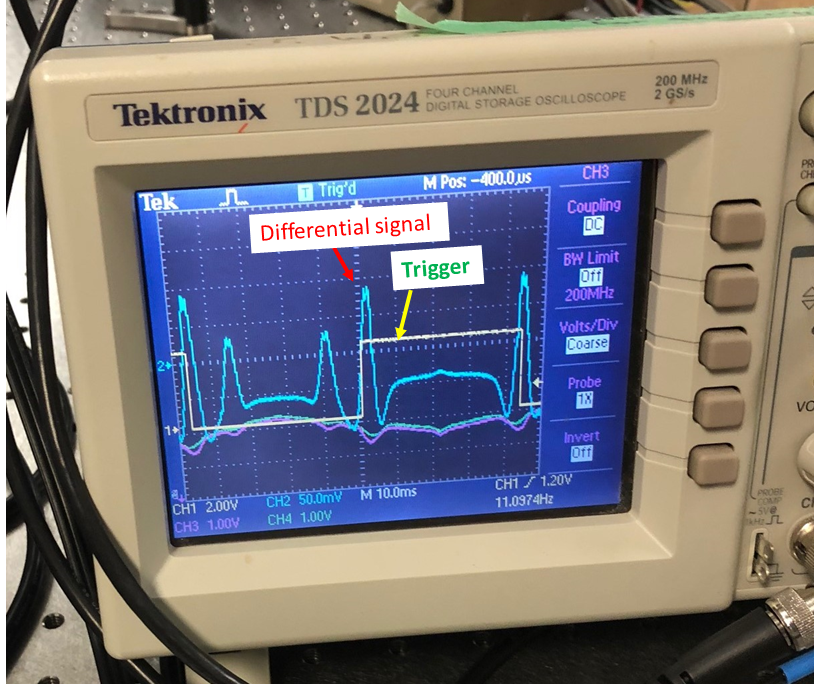
\includegraphics[width=0.7\linewidth]{figures/laser tune.png}
\caption{Oscilloscope trace of differential photodiode signal \label{fig:laser tune}}
\end{figure}
The output of the laser feedback controlyzer panel is connected to the computer where Digilock software was already installed. The output signal of the differential photodiode is fed into the controlyser panel main input. After connecting the DigiLock 110 we can turn on scan and navigate to the autolock screen at the bottom. Then the the portion of the spectrum that we tuned earlier will appear(see Fig \ref{fig:digilock}). Then we need to select the crosshairs tool which allow us to drag the crosshairs on the part of the spectrum that we want to tune to. Finally for successful laser locking we need to click and select "PID lock to slope". For most of the studies reported in this thesis we use the auto locking features of the DigiLock software.

\begin{table}[h]
\centering
\begin{tabular}{|l | l|}
\hline

\textbf{ Position}    & \textbf{Laser Power($\mu$W)} \\
\hline

AOM ~&  ~ ~ ~ ~ ~4000  \\

Pump beam ~  &  ~ ~ ~ ~ ~ 60  \\

Probe beam ~  &  ~ ~ ~ ~ ~ 22  \\
After Cell ~ &  ~ ~ ~ ~ ~ 18   \\

\hline
\end{tabular}
\caption{Adjusted laser power at several positions in the experiment.\label{table:laser power}}
\end{table}
\begin{figure}[h]
\centering
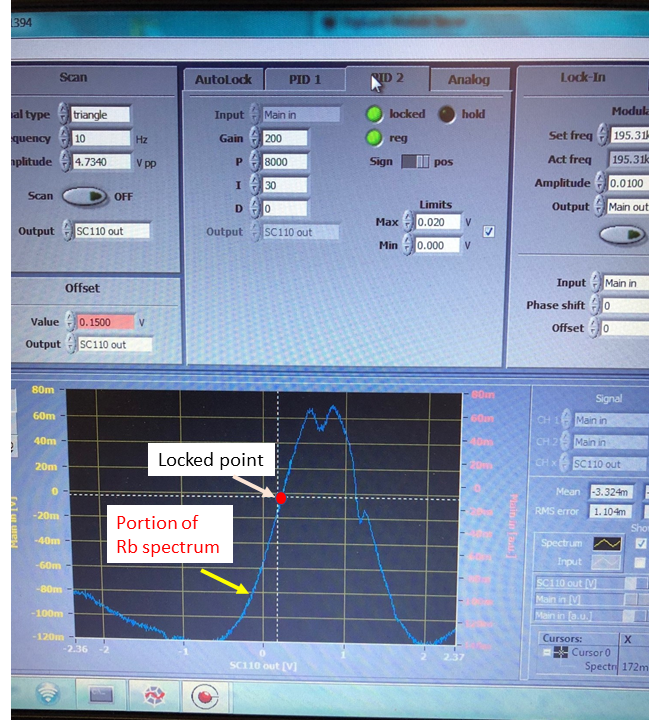
\includegraphics[width=0.6\linewidth]{figures/digilock.png}
\caption{digilock user interface\label{fig:digilock}}
\end{figure}
\section{Acousto-optic Modulator (AOM)\label{sec:AOM}}

The acousto-optic modulator offers a method of modulating the
amplitude of the light.
The AOM is used to modulate the amplitude of the pump beam. The pump beam is linearly polarized light, and so the amplitude
  is modulated at $2\omega_L$. This form of pumping generates a coherent precession of an axis of alignment in the atoms in the Rb cell. In FID mode, once the coherence has been sufficiently established, the AOM may be switched off in order to measure the precession frequency of the state using the probe beam.

 In principle, it contains an optically transparent medium (e.g glass, quartz) which has a piezoelectric transducer attached at the end that propagates acoustic waves within the medium. An RF signal needs to apply to the transducer to generate the acoustic wave. The compression and refraction of the sound waves result in periodic variations of the refractive index of the medium which then form a diffraction grating. Any incident laser beam will be diffracted by this grating generally provides a number of diffracted beams. The strength of the sound wave is directly related to the intensity of the defracted light. Depending on the interaction length L, laser wavelength $\lambda$ in the medium and the sound wavelength it is possible to operate AOM in two different modes, Raman-Nath regime and Bragg regime.

\begin{itemize}
\item In the Bragg regime~($L > \Lambda^2/\lambda$) the light beam enters the medium at one particular Bragg angle 
\begin{equation}
\theta_B=\frac{\lambda}{2\Lambda}
\end{equation}                                 
and only one diffraction order produce. This observed diffraction pattern generally consists of two diffraction maxima; these are the zeroth and the first orders. In this case the possible maximum intensity of the first order diffracted light is 100\%. Due to this relatively high efficiency, this first order can be used for amplitude modulation. For our atomic magnetometry setup we operated the AOM in the Bragg regime.
\end{itemize}
 For this experimental setup, an Isomet 1205C-1 AO Modulator  is used with an RF center frequency of 80 MHz. The AOM uses crystal Lead Molybdate (PbMo$0_4$) for the optical interaction medium and Lithium Niobate as the piezoelectric transducer. This AOM has a bandwidth of 80 MHz.  The amplitude modulating pulses are driven with an Isomet 532C-2 AO driver with video input range 0.0 V to 1.0 V. An Agilent 33522A function generator is used to regulate the  AOM driver. This amplitude modulation is done by a square wave modulation with a duty cycle of 1-10\%. For this specific model of AOM driver the RF rise/fall time is smaller than 6 nsec. Since the active aperture of the modulator is tiny (1mm) its very hard to focus the laser beam into it. In order to reach maximum deflected light intensity we need to adjust Bragg angle. In this setup, the achieved maximum intensity of the first order deflected light is 86$\%$. For  1~$\mu$T field the AOM operation frequency is 9335 Hz and the AOM driving frequency is 2034 Hz when the magnetometer operate at $0.2~ \mu$T .
\begin{figure}[h]
\centering
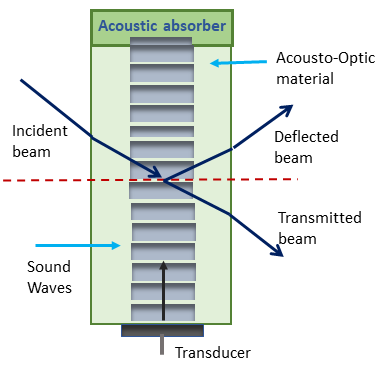
\includegraphics[width=0.7\linewidth]{figures/AOM}
\caption{Acousto-optic modulator}
\end{figure}

\section{Magnetic Shielding}
In precision magnetometry, magnetic shielding is required to achieve well characterized, stable magnetic field conditions independent of the earth’s magnetic fields and environmental perturbations. Shielding ratio T is a parameter to evaluate the efficiency of a shield which can be expressed as
\begin{equation}
 T = \frac{B_{in} }{B_0} 
\end{equation}

where $B_0$ is the homogeneous magnetic field in free space, and $B_{in}$ is the field induced in the presence of shield due to  $B_0$. Using multi-layer shielding is an efficient way to enhance shielding efficiency\cite{doe:website2} . The effectiveness of a multilayer shield with thin shells having wide gaps between them is same as the much heavier and more expensive thick, single layer shield.
The optimization of the air gaps between the shells is important to minimize the total size of a multilayer shield. When a coil is placed inside the innermost layer of passive shield the shield turns into a return yoke. As a result, the magnitude of field $B_0$ increase. A four layer $\mu$-metal magnetic shielding with nearly spherical geometry is used for this highly sensitive Rb magnetometer. $\mu$-metal is a very high permeability nickel based alloy, which is used for shielding low-frequency magnetic field. When the shape is close to a sphere we will get zero magnetic field inside independent of the outside field. The inner radius of the innermost shield is 18.44 cm, equal to its half-length. The radii and half-lengths of the progressively larger outer shields increase geometrically by a factor of 1.27. Each cylinder has two endcaps which possess a 7.5 cm diameter central hole\cite{Andalib:2016ahj}. A stove-pipe of length 5.5 cm is placed on each hole was designed to minimize leakage of external fields into the progressively shielded inner volumes. The magnetic shielding factors of each of the four cylindrical shells, and of various combinations of them, were measured and found to be consistent with $\mu_r \sim 20, 000$\cite{Martin:2014foa}
\begin{figure}[h]
\centering
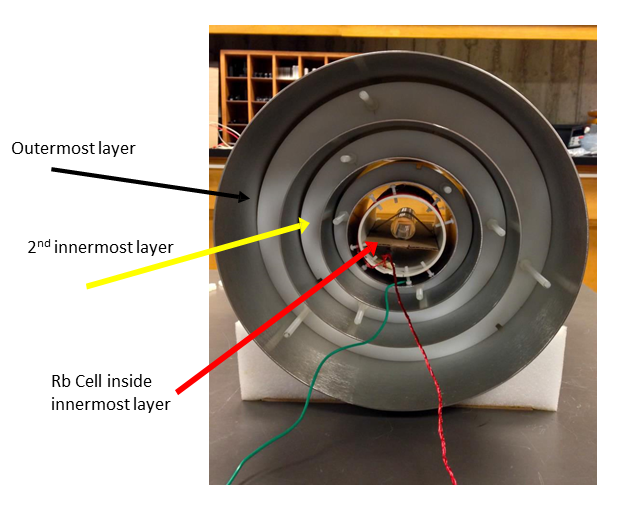
\includegraphics[width=1.0\linewidth]{figures/magnetic_shielding}
 \caption{Four layer $\mu$ -metal magnetic shielding.The diameter of each endcap is larger by 0.1 cm to fit over its corresponding cylinder. The hole diameter and stovepipe length for each endcap are the same. High density polyethylene spacers and nylon thread rods/nuts are used to hold the shields and end caps together.}
\end{figure}

\section{Degaussing system\label{sec:Degaussing}}
Our four layer $\mu$ metal magnetic shield is designed to minimize the magnetic field at the cell, but
magnetic hysteresis limits the magnetic field in any region to be exactly zero. Degaussing (demagnetizing) process is used to reduce the background magnetic field inside the shield. Although Rb cell is securely placed inside the four layer mu-metal shielding it is necessary to demagnetize the shield before every measurement session  to eliminate accidentally created local magnetizations.
Demagnetizing is achieved by winding a special coil around inner most layer of shielding  in toroidal configuration
and supplying the coil with oscillating current. An Agilent 3522A function generator  provides a ramped sinusoidal that controls a current supply driving the degaussing coil \cite{Martin:2014foa}. The wires going to the degaussing loop should be twisted together to avoid picking up or causing noise. Switch is opened to electrically disconnect the degaussing coil.
 
\begin{figure}[h]
\centering
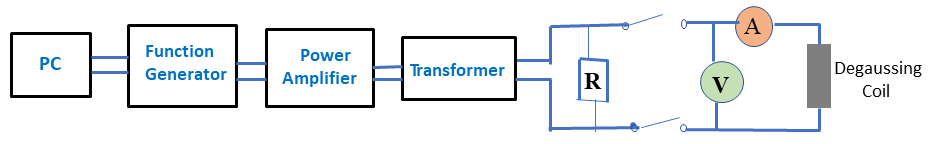
\includegraphics[width=1.0\linewidth]{figures/degaussing_system}
\caption{Schematic diagram of degaussing System}
\end{figure}

\section{Internal coil\label{sec:Internal coil}}
 For the Rb atomic magnetometer an internal coil referred as Z coil is used to provide the magnetic field. This coil produces uniform field in the ROI  of magnetic shielding, directed along the axis of light propagation direction (z-direction). The z-coil was wound on a 7.62 cm diameter, 20.32 cm long ABS plastic pipe. Seven turns of 26 AWG magnet wire were wound at 2.54 cm spacing, with 1.27 cm spacing from the magnetic faces of the endcaps of the innermost magnetic shield. The spacings were chosen so that, in the infinite permeability limit, and in the limit where the axial aperture holes in the endcaps are small, the boundary conditions would produce image currents forming an infinitely long solenoid. Two saddle coils were wound on the same cylinder in order to control transverse fields( along x and y) internally; these were normally disconnected during precision measurements. The internal coil system was calibrated using a three-axis fluxgate magnetometer at fields of ∼100 nT. This fluxgate was too large to fit through the end caps of the shield, so calibration
had to be performed without end caps. The calibration constant for z coil is 48nT/mA and the calibration constant for x and y coil is 25nT/mA. The calibration of the z-coil was verified using the NMOR magnetometer with an AM pump beam, and the known gyromagnetic ratios of Rb-85 and Rb-87. Homogeneity of the residual field and magnetic field generated by the coil system was measured by scanning a fluxgate magnetometer along the axis of the system with and without the coil energized. At a field of 1 $\mu$T, the axial field generated by the coil was uniform within the ROI to the $1\%$  level.

\section{Rb Cell}
When glass cell is used to store alkali atoms, the atomic mean free paths increase and alkali spins depolarize immediately after making non-elastic collision with the glass walls. Prolonging the atomic alignment is crucial to achieving ultra-narrow NMOR resonance widths. So it is necessary to prevent these non-elastic collisions for achieving the longer lifetimes of atomic ground state coherences \cite{PhysRevA.72.023401}\cite{Balabas:10}  \cite{doi:10.1063/1.3236649}. Two methods are currently in use to extent the atomic coherence lifetime. One of them is to add buffer gas to the cell containing alkali sample and the other method is to coat the inner walls of the cell with anti-relaxation materials. The advantage of using buffer gas is that it reduces the resonance width by extending the lifetime of coherence state. A paraffin-coated vapor cell containing  natural rubidium with stable isotopes $^{85}$Rb and $^{87}$Rb is used for this work. The reason behind using paraffin as a anti-relaxation coating is that it allow polarized atoms to bounce off the walls of a paraffin-coated cell $\sim 1000$ times before depolarizing \cite{PhysRev.147.41} \cite{PhysRevA.72.023401}. Coated cells have the advantages of providing larger optical rotation
signals, reducing the effect of magnetic field gradients on the spin polarization lifetime,
and lowering the power requirements of the lasers used for pumping and probing. The vapor cell is cylindrical, 5 cm long and 5 cm in diameter with optical
flats on the ends. The cell was provided by D. Budker, having been prepared in
a fashion similar to the cells described in Ref.\cite{PhysRevA.72.023401}. The cell was characterized
using a method similar to Ref. \cite{PhysRevA.72.023401}, by measuring the relaxation of longitudinal
polarization using optical rotation as a probe. The long time component of the relaxation was thereby found to decay with a time scale of 60 ms.  Longer relaxation time indicates good quality of cell. The temperature of the vapour cell was controlled by the ambient temperature of the surrounding room (∼ 21 $\degree$). Transmitted light was analyzed for optical rotation by a balanced polarimeter system containing a Wollaston prism and a Newport model 2307 balanced photo receiver. The power delivered to the vapour cell was typically 15 $\mu$W, measured periodically using a Newport model 818-SL power meter inserted into the
beamline. 
\begin{figure}[h]
\centering
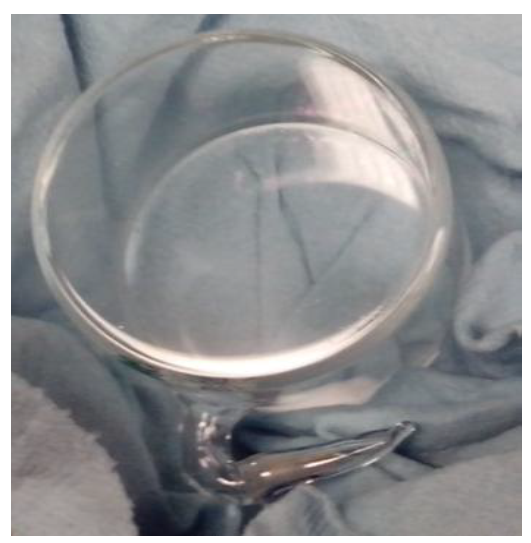
\includegraphics[width=0.5\linewidth]{figures/cell}
\caption{Paraffin coated Rb cell}
\end{figure}
\section{Lock in Amplifier}
SR830 DSP Lock in Amplifier is a elementary part in the DAQ system of Rb magnetometry. It can measure very  small voltages. The most attractive feature of a lock in amplifier is that it is able to suppress all noise contributions which differ from the reference frequency. A reference signal is applied to the lock-in amplifier which is usually done by an external oscillator which passes a discriminator. In this magnetometry setup sync output of a function generator is used as external reference signal for force oscillation scan. The external reference signal is phase locked to an internal reference frequency, provided internal oscillator of the lock-in.Since a lock-in amplifier has two phase sensitive detectors we obtain two output signals. During the process of phase sensitive detection (PSD), the reference signal is first multiplied with the real input signal  and in a second stage, the real input signal is multiplied by
the lock-in reference signal with a phase shift of $90\degree$. Then a lowpass filter is used to filter both signals. The first one is referred to as X output and the 2nd output signal is referred to as Y output. X output is knows as in phase component and the Y output is called out of phase component.


\section{Signal Processing\label{sec:Signal Processing}}
Sensitive magnetometry requires detection of extremely small optical rotation angles. There are numerous methods for detecting the optical rotation of the probe beam.  we instead use the balanced polarimetry technique.  After the cell the probe beam passes through a polarizing beamsplitter set at 45\degree~to the initial polarization direction resulting in two separate beams with individual intensities given by 
\begin{equation}
I_1 = I_0\sin^2(\theta-\frac{\pi}{4})
\end{equation}

\begin{equation}
I_2 = I_0 \cos^2(\theta-\frac{\pi}{4})   
\end{equation}

such that $I_1 + I_2 = I_0$, and the intensities are balanced when $\theta = 0$ and unbalanced otherwise. 
For small rotations $\theta << 1$ in terms of power we can write,
\begin{equation}
  \theta \approx \frac{P_1-P_2}{2(P_1-P_2)}  
\end{equation}

where $P_1$ and $P_2$ represent signals of the two photodiodes in the polarimeter. The differential value is acquired with a lock-in amplifier (LIA) referenced to the pump beam modulation provided by a function generator. The demodulated signal from the LIA is acquired by a personal computer for analysis. 

